\documentclass[man,floatsintext]{apa6}
\usepackage{lmodern}
\usepackage{amssymb,amsmath}
\usepackage{ifxetex,ifluatex}
\usepackage{fixltx2e} % provides \textsubscript
\ifnum 0\ifxetex 1\fi\ifluatex 1\fi=0 % if pdftex
  \usepackage[T1]{fontenc}
  \usepackage[utf8]{inputenc}
\else % if luatex or xelatex
  \ifxetex
    \usepackage{mathspec}
  \else
    \usepackage{fontspec}
  \fi
  \defaultfontfeatures{Ligatures=TeX,Scale=MatchLowercase}
\fi
% use upquote if available, for straight quotes in verbatim environments
\IfFileExists{upquote.sty}{\usepackage{upquote}}{}
% use microtype if available
\IfFileExists{microtype.sty}{%
\usepackage{microtype}
\UseMicrotypeSet[protrusion]{basicmath} % disable protrusion for tt fonts
}{}
\usepackage{hyperref}
\PassOptionsToPackage{usenames,dvipsnames}{color} % color is loaded by hyperref
\hypersetup{unicode=true,
            pdftitle={RMarkdown based APA Manuscript with `papaja'},
            pdfauthor={Jenny Rieck~\& Derek Beaton},
            pdfkeywords={reproducible, manuscript, multivariate, APA, papaja, knitr, R, Rmarkdown},
            colorlinks=true,
            linkcolor=blue,
            citecolor=Blue,
            urlcolor=Blue,
            breaklinks=true}
\urlstyle{same}  % don't use monospace font for urls
\usepackage{color}
\usepackage{fancyvrb}
\newcommand{\VerbBar}{|}
\newcommand{\VERB}{\Verb[commandchars=\\\{\}]}
\DefineVerbatimEnvironment{Highlighting}{Verbatim}{commandchars=\\\{\}}
% Add ',fontsize=\small' for more characters per line
\usepackage{framed}
\definecolor{shadecolor}{RGB}{248,248,248}
\newenvironment{Shaded}{\begin{snugshade}}{\end{snugshade}}
\newcommand{\AlertTok}[1]{\textcolor[rgb]{0.94,0.16,0.16}{#1}}
\newcommand{\AnnotationTok}[1]{\textcolor[rgb]{0.56,0.35,0.01}{\textbf{\textit{#1}}}}
\newcommand{\AttributeTok}[1]{\textcolor[rgb]{0.77,0.63,0.00}{#1}}
\newcommand{\BaseNTok}[1]{\textcolor[rgb]{0.00,0.00,0.81}{#1}}
\newcommand{\BuiltInTok}[1]{#1}
\newcommand{\CharTok}[1]{\textcolor[rgb]{0.31,0.60,0.02}{#1}}
\newcommand{\CommentTok}[1]{\textcolor[rgb]{0.56,0.35,0.01}{\textit{#1}}}
\newcommand{\CommentVarTok}[1]{\textcolor[rgb]{0.56,0.35,0.01}{\textbf{\textit{#1}}}}
\newcommand{\ConstantTok}[1]{\textcolor[rgb]{0.00,0.00,0.00}{#1}}
\newcommand{\ControlFlowTok}[1]{\textcolor[rgb]{0.13,0.29,0.53}{\textbf{#1}}}
\newcommand{\DataTypeTok}[1]{\textcolor[rgb]{0.13,0.29,0.53}{#1}}
\newcommand{\DecValTok}[1]{\textcolor[rgb]{0.00,0.00,0.81}{#1}}
\newcommand{\DocumentationTok}[1]{\textcolor[rgb]{0.56,0.35,0.01}{\textbf{\textit{#1}}}}
\newcommand{\ErrorTok}[1]{\textcolor[rgb]{0.64,0.00,0.00}{\textbf{#1}}}
\newcommand{\ExtensionTok}[1]{#1}
\newcommand{\FloatTok}[1]{\textcolor[rgb]{0.00,0.00,0.81}{#1}}
\newcommand{\FunctionTok}[1]{\textcolor[rgb]{0.00,0.00,0.00}{#1}}
\newcommand{\ImportTok}[1]{#1}
\newcommand{\InformationTok}[1]{\textcolor[rgb]{0.56,0.35,0.01}{\textbf{\textit{#1}}}}
\newcommand{\KeywordTok}[1]{\textcolor[rgb]{0.13,0.29,0.53}{\textbf{#1}}}
\newcommand{\NormalTok}[1]{#1}
\newcommand{\OperatorTok}[1]{\textcolor[rgb]{0.81,0.36,0.00}{\textbf{#1}}}
\newcommand{\OtherTok}[1]{\textcolor[rgb]{0.56,0.35,0.01}{#1}}
\newcommand{\PreprocessorTok}[1]{\textcolor[rgb]{0.56,0.35,0.01}{\textit{#1}}}
\newcommand{\RegionMarkerTok}[1]{#1}
\newcommand{\SpecialCharTok}[1]{\textcolor[rgb]{0.00,0.00,0.00}{#1}}
\newcommand{\SpecialStringTok}[1]{\textcolor[rgb]{0.31,0.60,0.02}{#1}}
\newcommand{\StringTok}[1]{\textcolor[rgb]{0.31,0.60,0.02}{#1}}
\newcommand{\VariableTok}[1]{\textcolor[rgb]{0.00,0.00,0.00}{#1}}
\newcommand{\VerbatimStringTok}[1]{\textcolor[rgb]{0.31,0.60,0.02}{#1}}
\newcommand{\WarningTok}[1]{\textcolor[rgb]{0.56,0.35,0.01}{\textbf{\textit{#1}}}}
\usepackage{graphicx,grffile}
\makeatletter
\def\maxwidth{\ifdim\Gin@nat@width>\linewidth\linewidth\else\Gin@nat@width\fi}
\def\maxheight{\ifdim\Gin@nat@height>\textheight\textheight\else\Gin@nat@height\fi}
\makeatother
% Scale images if necessary, so that they will not overflow the page
% margins by default, and it is still possible to overwrite the defaults
% using explicit options in \includegraphics[width, height, ...]{}
\setkeys{Gin}{width=\maxwidth,height=\maxheight,keepaspectratio}
\IfFileExists{parskip.sty}{%
\usepackage{parskip}
}{% else
\setlength{\parindent}{0pt}
\setlength{\parskip}{6pt plus 2pt minus 1pt}
}
\setlength{\emergencystretch}{3em}  % prevent overfull lines
\providecommand{\tightlist}{%
  \setlength{\itemsep}{0pt}\setlength{\parskip}{0pt}}
\setcounter{secnumdepth}{0}
% Redefines (sub)paragraphs to behave more like sections
\ifx\paragraph\undefined\else
\let\oldparagraph\paragraph
\renewcommand{\paragraph}[1]{\oldparagraph{#1}\mbox{}}
\fi
\ifx\subparagraph\undefined\else
\let\oldsubparagraph\subparagraph
\renewcommand{\subparagraph}[1]{\oldsubparagraph{#1}\mbox{}}
\fi

%%% Use protect on footnotes to avoid problems with footnotes in titles
\let\rmarkdownfootnote\footnote%
\def\footnote{\protect\rmarkdownfootnote}


  \title{RMarkdown based APA Manuscript with `papaja'}
    \author{Jenny Rieck\textsuperscript{1}~\& Derek Beaton\textsuperscript{1}}
    \date{}
  
\shorttitle{RMD paper via papaja}
\affiliation{
\vspace{0.5cm}
\textsuperscript{1} Rotman Research Institute}
\keywords{reproducible, manuscript, multivariate, APA, papaja, knitr, R, Rmarkdown}
\usepackage{csquotes}
\usepackage{upgreek}
\captionsetup{font=singlespacing,justification=justified}

\usepackage{longtable}
\usepackage{lscape}
\usepackage{multirow}
\usepackage{tabularx}
\usepackage[flushleft]{threeparttable}
\usepackage{threeparttablex}

\newenvironment{lltable}{\begin{landscape}\begin{center}\begin{ThreePartTable}}{\end{ThreePartTable}\end{center}\end{landscape}}

\makeatletter
\newcommand\LastLTentrywidth{1em}
\newlength\longtablewidth
\setlength{\longtablewidth}{1in}
\newcommand{\getlongtablewidth}{\begingroup \ifcsname LT@\roman{LT@tables}\endcsname \global\longtablewidth=0pt \renewcommand{\LT@entry}[2]{\global\advance\longtablewidth by ##2\relax\gdef\LastLTentrywidth{##2}}\@nameuse{LT@\roman{LT@tables}} \fi \endgroup}
\usepackage{float}
\usepackage{bbold}
\usepackage{subfig}
\usepackage{graphicx}
\usepackage[utf8]{inputenc}
\usepackage[T1]{fontenc}
\usepackage{booktabs}
\usepackage{algorithm2e}
\usepackage{caption}

\authornote{We can include author notes for, e.g., attribution
of data or expanding on roles/locations.

}

\abstract{
This is a short example of a completely reproducible manuscript made
entirely in RStudio with RMarkdown and various R scripts, functions, and
packages.


}

\usepackage{amsthm}
\newtheorem{theorem}{Theorem}[section]
\newtheorem{lemma}{Lemma}[section]
\theoremstyle{definition}
\newtheorem{definition}{Definition}[section]
\newtheorem{corollary}{Corollary}[section]
\newtheorem{proposition}{Proposition}[section]
\theoremstyle{definition}
\newtheorem{example}{Example}[section]
\theoremstyle{definition}
\newtheorem{exercise}{Exercise}[section]
\theoremstyle{remark}
\newtheorem*{remark}{Remark}
\newtheorem*{solution}{Solution}
\begin{document}
\maketitle

\hypertarget{introduction}{%
\section{Introduction}\label{introduction}}

The aim of this RMarkdown example is to show how to write a reproducible
manuscript, which includes numerous bells-and-whistles---with
contributions from \texttt{R}, \texttt{Python}, RMarkdown, and
\texttt{LaTeX}. This \enquote{manuscript} will include only the best
(nicest looking) parts from \texttt{1\_a\_Simple\_RMarkdown\_PDF.Rmd}

In order to help make this manuscript look nicer, we are changing some
of the YAML (\enquote{yet another markup language}) header options, so
that we remove line numbers, and allow for tables \& figures to appear
in text, as opposed to the end.

\hypertarget{methods}{%
\section{Methods}\label{methods}}

We first make our data with R. This will be followed by a paragraph
break because this text precedes a chunk.

Then call off to python for the \texttt{.describe()} method. This, too,
will be followed by a paragraph break because this text precedes a
chunk.

And then pass the \texttt{desc} object back to \texttt{R} and use the
\texttt{kable()} and \texttt{kableExtra} packages to make a nice table
of summary statistics for the measures of interest. In this particular
part, we also show the code chunk. Furthermore, some particular
packages---such as \texttt{papaja}---and certain advanced features from
\texttt{LaTeX} require the use of
\texttt{results=\textquotesingle{}asis\textquotesingle{}} in chunk
header.

\begin{Shaded}
\begin{Highlighting}[]
\KeywordTok{apa_table}\NormalTok{(py}\OperatorTok{$}\NormalTok{desc, }\DataTypeTok{caption =} \StringTok{"A descriptive statistics table."}\NormalTok{, }
    \DataTypeTok{note =} \StringTok{"This formatted through LaTeX via papaja::apa_table() from a python object from the .describe() method, loaded from data in R and written through RMarkdown."}\NormalTok{)}
\end{Highlighting}
\end{Shaded}

\begin{table}[tbp]
\begin{center}
\begin{threeparttable}
\caption{\label{tab:python_describe_via_kable}A descriptive statistics table.}
\begin{tabular}{lllllll}
\toprule
 & \multicolumn{1}{c}{AGE} & \multicolumn{1}{c}{MOCA} & \multicolumn{1}{c}{CDRSB} & \multicolumn{1}{c}{WholeBrain} & \multicolumn{1}{c}{Hippocampus} & \multicolumn{1}{c}{MidTemp}\\
\midrule
count & 665.00 & 665.00 & 665.00 & 665.00 & 665.00 & 665.00\\
mean & 71.92 & 23.89 & 1.20 & 1,057,025.55 & 7,149.61 & 20,301.93\\
std & 6.87 & 3.28 & 1.34 & 103,672.74 & 1,086.04 & 2,675.57\\
min & 55.00 & 16.00 & 0.00 & 817,421.23 & 3,731.00 & 12,213.00\\
25\% & 67.20 & 22.00 & 0.00 & 984,409.91 & 6,510.00 & 18,535.00\\
50\% & 71.90 & 24.00 & 1.00 & 1,051,621.33 & 7,223.00 & 20,186.00\\
75\% & 76.60 & 26.00 & 2.00 & 1,120,569.50 & 7,834.00 & 22,088.00\\
max & 89.60 & 30.00 & 5.50 & 1,486,035.64 & 10,602.00 & 32,189.00\\
\bottomrule
\addlinespace
\end{tabular}
\begin{tablenotes}[para]
\normalsize{\textit{Note.} This formatted through LaTeX via papaja::apa\_table() from a python object from the .describe() method, loaded from data in R and written through RMarkdown.}
\end{tablenotes}
\end{threeparttable}
\end{center}
\end{table}

\hypertarget{procedure}{%
\subsection{Procedure}\label{procedure}}

Next we are going to use more features from \texttt{LaTeX}, including
various additional \texttt{LaTeX} packages that we define in the YAML
header. We can use a number of \texttt{LaTeX} features like inline
calls, numbered equations, and, for eaxmple, algorithms. We will use
each of those features to describe the covSTATIS method (see also
\href{https://github.com/jennyrieck/C-MARINeR}{our covSTATIS project
repository}). Our description of covSTATIS is extremely truncated here
and is only meant to illustrate features of writing a manuscript in
RMarkdown.

CovSTATIS is a multi-table principal components analysis, specifically
designed to integrate and analyze multiple correlation or covariance
matrices. Each correlation matrix---\({\bf R}_{[k]}\)---is
double-centered by way of a centering matrix as
\({\boldsymbol \Xi} = \mathbf{I} - \mathbf{1}(I^{-1})\mathbf{1}^{T}\) as

\begin{equation}
{\bf S}_{[k]} = \frac{1}{2}{\boldsymbol \Xi}{\bf R}_{[k]}{\boldsymbol \Xi}.
\label{eq:double_center}
\end{equation}

After we perform the double-centering in Eq. @ref(eq:double\_center), we
then compute \(\alpha\) weights of each matrix where first we vectorize
each \({\bf S}_{[k]}\) and storing those each column vector in a new
matrix as
\(\mathbf{Z} = [ \mathrm{vec\{ {\bf S}_{[1]}, \dots, {\bf S}_{[k]}, \dots, {\bf S}_{[K]} \}} ]\)
and then decompose \(\mathbf{Z}\) with the singular value decomposition
(SVD):

\begin{equation}
\mathbf{Z} = \mathbf{U}\boldsymbol{\Delta}\mathbf{V}^{T}.
\end{equation}

The \(alpha\) weights are
\(\boldsymbol{\alpha} = \mathbf{v}_{1} \times (\mathbf{v}_{1}^{T}\mathbf{1})^{-1}\).
We then compute the compromise cross-product matrix as
\(\mathbf{S}_{[+]} = \sum\limits_{i=1}^K \alpha_{k}\mathbf{S}_{[k]}\),
and finally decompose \(\mathbf{S}_{[+]}\) with the eigenvalue
decomposition (EVD) as

\begin{equation}
\mathbf{S}_{[+]} = \mathbf{Q}\boldsymbol{\Lambda}\mathbf{Q}^{T}.
\end{equation}

We can also outline these steps algorithmically as

\RestyleAlgo{boxed}
\begin{algorithm}
\DontPrintSemicolon
\SetAlgoLined
\KwResult{Decomposition of the compromise matrix---$\mathbf{S}_{[+]}$---in covSTATIS}
\SetKwInOut{Input}{Input}\SetKwInOut{Output}{Output}
\Input{$[{\bf R}_{[1]} ... {\bf R}_{[k]} ... {\bf R}_{[K]}]$}
\Output{$\mathbf{Q}$, $\boldsymbol{\Lambda}$}
Define $\mathbf{S}_{[+]} = \mathbf{0}$
\BlankLine
\For{$k=1, \dots, K$}{
    ${\bf S}_{[k]} \leftarrow \frac{1}{2}{\boldsymbol \Xi}{\bf R}_{[k]}{\boldsymbol \Xi}$
}
$\mathbf{Z} \leftarrow [ \mathrm{vec\{ {\bf S}_{[1]}, \dots, {\bf S}_{[k]}, \dots, {\bf S}_{[K]}   \}} ]$

$\mathbf{U}\boldsymbol{\Delta}\mathbf{V}^{T} \leftarrow \mathrm{SVD(}\mathbf{Z}\mathrm{)}$

$\boldsymbol{\alpha} \leftarrow \mathbf{v}_{1}  \times (\mathbf{v}_{1}^{T}\mathbf{1})^{-1}$

\For{$k=1, \dots, K$}{
    $\mathbf{S}_{[+]} \leftarrow \mathbf{S}_{[+]} + (\mathbf{S}_{[k]} \times \alpha_{[k]})$
}

$\mathbf{Q}\boldsymbol{\Lambda}\mathbf{Q}^{T} \leftarrow \mathrm{EVD(}\mathbf{S}_{[+]}\mathrm{)}$
\caption{CovSTATIS algorithm}
\label{algo:covstatis}
\end{algorithm}

\hypertarget{data-analysis}{%
\subsection{Data analysis}\label{data-analysis}}

The \texttt{papaja} package includes the ability to generate a
bibliography directly from all the loaded packages (via
\texttt{cite\_r()}). This document includes R (Version 3.5.1; R Core
Team, 2018) and the R-packages \emph{covstatis} (Version 0.1.0.0; Rieck
\& Beaton, n.d.), \emph{dplyr} (Version 0.7.6; Wickham et al., 2018),
\emph{ExPosition} (Version 2.8.23; Beaton et al., 2014a),
\emph{factoextra} (Version 1.0.5; Kassambara \& Mundt, 2017),
\emph{forcats} (Version 0.3.0; Wickham, 2018a), \emph{ggplot2} (Version
3.0.0; Wickham, 2016), \emph{gridExtra} (Version 2.3; Auguie, 2017),
\emph{GSVD} (Version 0.2.0; Beaton, n.d.), \emph{here} (Version 0.1;
Müller, 2017), \emph{kableExtra} (Version 0.9.0; Zhu, 2018),
\emph{knitr} (Version 1.23.2; Xie, 2015), \emph{ours} (Version
0.0.0.9000; Sunderland \& Beaton, n.d.), \emph{papaja} (Version
0.1.0.9842; Aust \& Barth, 2018), \emph{prettyGraphs} (Version 2.1.6;
Beaton et al., 2014b), \emph{purrr} (Version 0.2.5; Henry \& Wickham,
2018), \emph{readr} (Version 1.1.1; Wickham et al., 2017),
\emph{reticulate} (Version 1.9; Allaire, Ushey, \& Tang, 2018),
\emph{RevoUtils} (Version 11.0.1; Corporation, 2018b, 2018a),
\emph{RevoUtilsMath} (Version 11.0.0; Corporation, 2018a),
\emph{stringr} (Version 1.3.1; Wickham, 2018b), \emph{tibble} (Version
1.4.2; Müller \& Wickham, 2018), \emph{tidyr} (Version 0.8.1; Wickham \&
Henry, 2018), and \emph{tidyverse} (Version 1.2.1; Wickham, 2017) for
all our analyses.

\hypertarget{results}{%
\section{Results}\label{results}}

Like in the other example RMarkdown file, we call off to an \texttt{R}
script

\begin{figure}[H]

{\centering 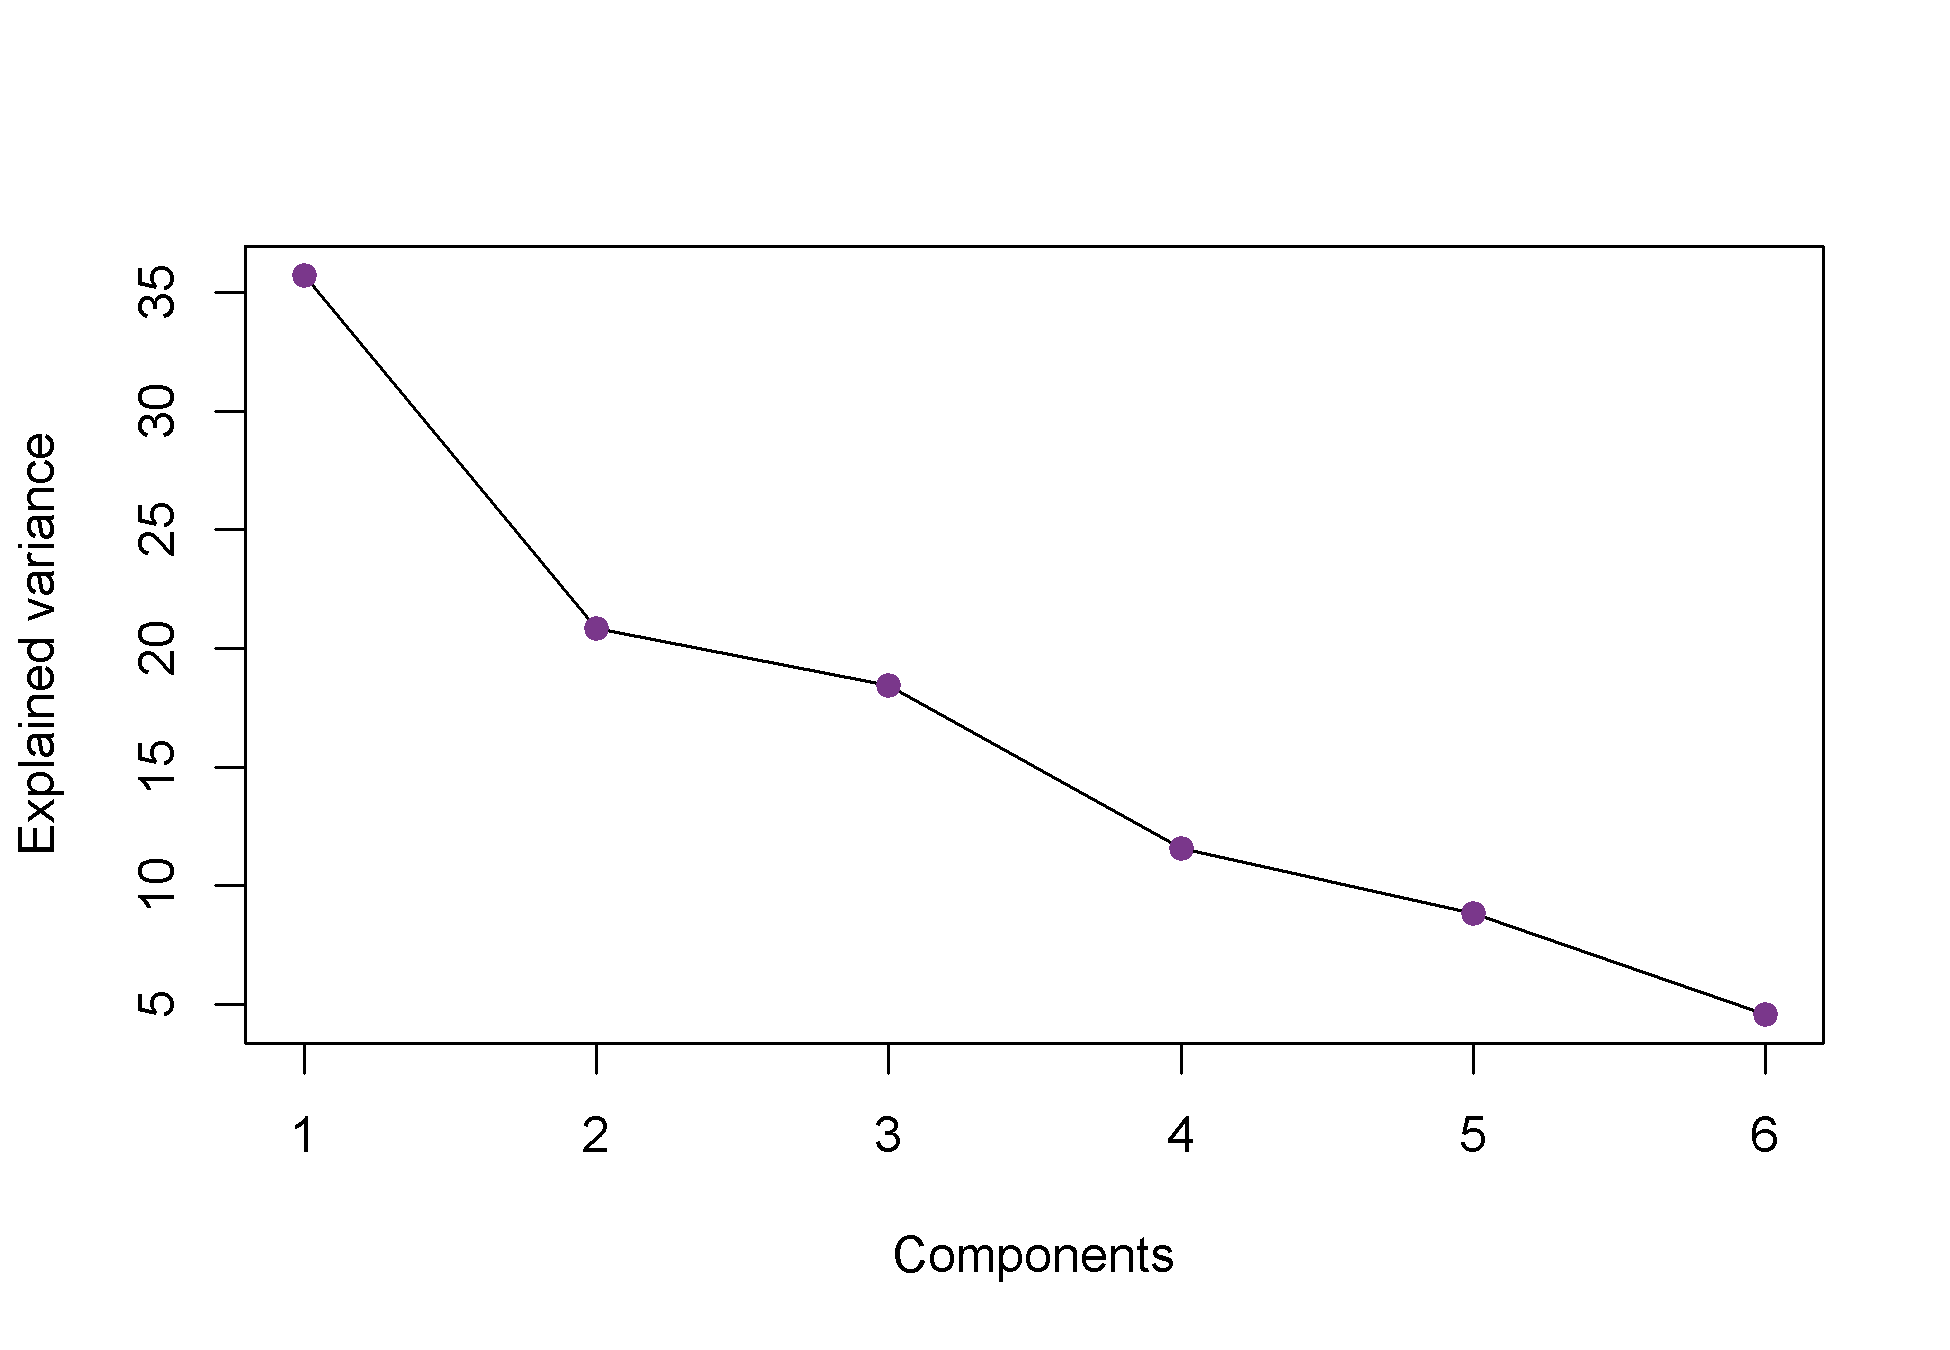
\includegraphics{3_RMarkdown_APA_Manuscript_files/figure-latex/scree-1} 

}

\caption{Scree plot of the covSTATIS compromise results.}\label{fig:scree}
\end{figure}

\begin{figure}[H]

{\centering 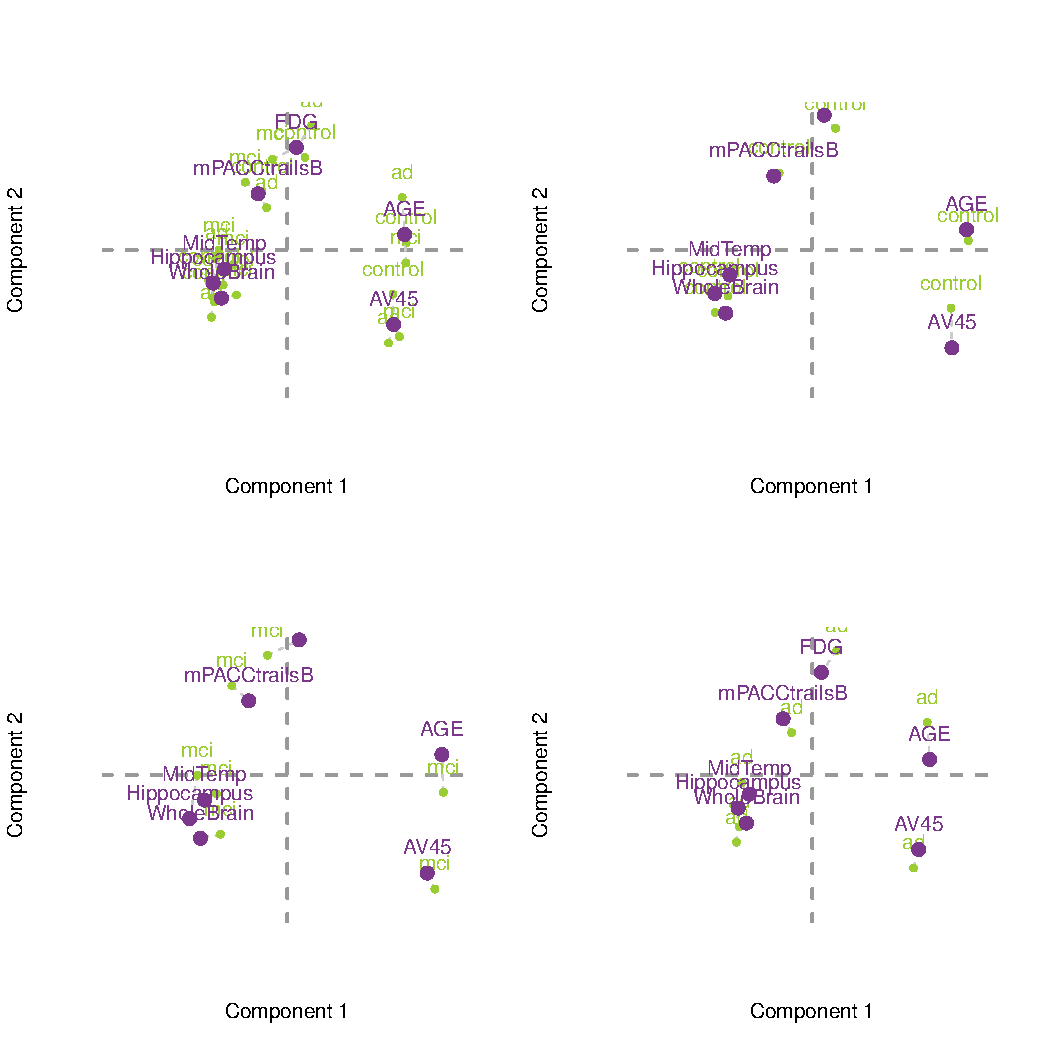
\includegraphics{3_RMarkdown_APA_Manuscript_files/figure-latex/unnamed-chunk-1-1} 

}

\caption{Component maps with the compromise (purple) and each group's results (green) projected onto the compromise.}\label{fig:unnamed-chunk-1}
\end{figure}

\hypertarget{discussion}{%
\section{Discussion}\label{discussion}}

This example manuscript provides an illustrative view of how to write a
reproducible paper in RMarkdown with the help of various external tools
(e.g., \texttt{LaTeX}, \texttt{Python}) and \texttt{R}/RStudio tools.
References can be included in two ways: through \texttt{LaTeX}
bibliography files or through the use of additional \texttt{R} packages
and Rstudio plugins, such as
\href{https://github.com/crsh/citr}{\texttt{citr}}.

\newpage

\hypertarget{references}{%
\section{References}\label{references}}

\begingroup
\setlength{\parindent}{-0.5in}
\setlength{\leftskip}{0.5in}

\hypertarget{refs}{}
\leavevmode\hypertarget{ref-R-reticulate}{}%
Allaire, J., Ushey, K., \& Tang, Y. (2018). \emph{Reticulate: Interface
to 'python'}. Retrieved from
\url{https://CRAN.R-project.org/package=reticulate}

\leavevmode\hypertarget{ref-R-gridExtra}{}%
Auguie, B. (2017). \emph{GridExtra: Miscellaneous functions for "grid"
graphics}. Retrieved from
\url{https://CRAN.R-project.org/package=gridExtra}

\leavevmode\hypertarget{ref-R-papaja}{}%
Aust, F., \& Barth, M. (2018). \emph{papaja: Create APA manuscripts with
R Markdown}. Retrieved from \url{https://github.com/crsh/papaja}

\leavevmode\hypertarget{ref-R-GSVD}{}%
Beaton, D. (n.d.). \emph{GSVD: The generalized singular value
decomposition}.

\leavevmode\hypertarget{ref-R-ExPosition}{}%
Beaton, D., Fatt, C. R. C., \& Abdi, H. (2014a). An ExPosition of
multivariate analysis with the singular value decomposition in R.
\emph{Computational Statistics \& Data Analysis}, \emph{72}(0),
176--189. \url{https://doi.org/10.1016/j.csda.2013.11.006}

\leavevmode\hypertarget{ref-R-prettyGraphs}{}%
Beaton, D., Fatt, C. R. C., \& Abdi, H. (2014b). An ExPosition of
multivariate analysis with the singular value decomposition in R.
\emph{Computational Statistics \& Data Analysis}, \emph{72}(0),
176--189. \url{https://doi.org/10.1016/j.csda.2013.11.006}

\leavevmode\hypertarget{ref-R-RevoUtilsMath}{}%
Corporation, M. (2018a). \emph{RevoUtilsMath: Microsoft r services math
utilities package}.

\leavevmode\hypertarget{ref-R-RevoUtils}{}%
Corporation, M. (2018b). \emph{RevoUtils: Microsoft r utility package}.

\leavevmode\hypertarget{ref-R-purrr}{}%
Henry, L., \& Wickham, H. (2018). \emph{Purrr: Functional programming
tools}. Retrieved from \url{https://CRAN.R-project.org/package=purrr}

\leavevmode\hypertarget{ref-R-factoextra}{}%
Kassambara, A., \& Mundt, F. (2017). \emph{Factoextra: Extract and
visualize the results of multivariate data analyses}. Retrieved from
\url{https://CRAN.R-project.org/package=factoextra}

\leavevmode\hypertarget{ref-R-here}{}%
Müller, K. (2017). \emph{Here: A simpler way to find your files}.
Retrieved from \url{https://CRAN.R-project.org/package=here}

\leavevmode\hypertarget{ref-R-tibble}{}%
Müller, K., \& Wickham, H. (2018). \emph{Tibble: Simple data frames}.
Retrieved from \url{https://CRAN.R-project.org/package=tibble}

\leavevmode\hypertarget{ref-R-base}{}%
R Core Team. (2018). \emph{R: A language and environment for statistical
computing}. Vienna, Austria: R Foundation for Statistical Computing.
Retrieved from \url{https://www.R-project.org/}

\leavevmode\hypertarget{ref-R-covstatis}{}%
Rieck, J., \& Beaton, D. (n.d.). \emph{Covstatis: CovSTATIS}.

\leavevmode\hypertarget{ref-R-ours}{}%
Sunderland, K., \& Beaton, D. (n.d.). \emph{Ours: OUtliers and robust
structures}.

\leavevmode\hypertarget{ref-R-ggplot2}{}%
Wickham, H. (2016). \emph{Ggplot2: Elegant graphics for data analysis}.
Springer-Verlag New York. Retrieved from \url{http://ggplot2.org}

\leavevmode\hypertarget{ref-R-tidyverse}{}%
Wickham, H. (2017). \emph{Tidyverse: Easily install and load the
'tidyverse'}. Retrieved from
\url{https://CRAN.R-project.org/package=tidyverse}

\leavevmode\hypertarget{ref-R-forcats}{}%
Wickham, H. (2018a). \emph{Forcats: Tools for working with categorical
variables (factors)}. Retrieved from
\url{https://CRAN.R-project.org/package=forcats}

\leavevmode\hypertarget{ref-R-stringr}{}%
Wickham, H. (2018b). \emph{Stringr: Simple, consistent wrappers for
common string operations}. Retrieved from
\url{https://CRAN.R-project.org/package=stringr}

\leavevmode\hypertarget{ref-R-dplyr}{}%
Wickham, H., François, R., Henry, L., \& Müller, K. (2018). \emph{Dplyr:
A grammar of data manipulation}. Retrieved from
\url{https://CRAN.R-project.org/package=dplyr}

\leavevmode\hypertarget{ref-R-tidyr}{}%
Wickham, H., \& Henry, L. (2018). \emph{Tidyr: Easily tidy data with
'spread()' and 'gather()' functions}. Retrieved from
\url{https://CRAN.R-project.org/package=tidyr}

\leavevmode\hypertarget{ref-R-readr}{}%
Wickham, H., Hester, J., \& Francois, R. (2017). \emph{Readr: Read
rectangular text data}. Retrieved from
\url{https://CRAN.R-project.org/package=readr}

\leavevmode\hypertarget{ref-R-knitr}{}%
Xie, Y. (2015). \emph{Dynamic documents with R and knitr} (2nd ed.).
Boca Raton, Florida: Chapman; Hall/CRC. Retrieved from
\url{https://yihui.name/knitr/}

\leavevmode\hypertarget{ref-R-kableExtra}{}%
Zhu, H. (2018). \emph{KableExtra: Construct complex table with 'kable'
and pipe syntax}. Retrieved from
\url{https://CRAN.R-project.org/package=kableExtra}

\endgroup


\end{document}
